\documentclass[%
  a4paper,%                                        % DIN A4
  oneside,%                                        % einseitiger Druck
  12pt,%                                           % 12pt Schriftgröße
]{article}

%\usepackage{ifpdf}

%\usepackage[english]{babel}

% UTF8 input
\usepackage[utf8]{inputenc}

% grafics
\usepackage{graphicx}
%\usepackage{picinpar}

% others
%\usepackage{parcolumns}
%\usepackage[font=footnotesize,format=plain,labelfont=bf]{caption}
%\usepackage{paralist}
\usepackage{url}
\usepackage{array}
\usepackage{tocloft}
\usepackage{color}
\usepackage{listings}
\usepackage{xspace}
\usepackage{tabularx}
\usepackage{hyperref}

\usepackage{fancyhdr}

\usepackage{multicol}

\usepackage{hevea}

\usepackage{cmbright}
\usepackage{txfonts}
\usepackage[scaled=.90]{helvet}
\usepackage{courier}
%\usepackage{natbib}

%\usepackage{lmodern}
%\usepackage{newcent}

%\renewcommand{\ttdefault}{lmtt}

%\usepackage{fontspec}
%\defaultfontfeatures{Mapping=tex-text}  % For archaic input (e.g. convert -- to en-dash)
%\setmainfont{Times New Roman}                 % Computer Modern Unicode font
%\setmonofont{Anonymous Pro}
%\setsansfont{Times New Roman}

% par. settings
\parindent 0pt
\parskip 8pt

\definecolor{blue}{rgb}{0,0,1}
\definecolor{violet}{rgb}{0.5,0,0.5}

\definecolor{darkred}{rgb}{0.5,0,0}
\definecolor{darkblue}{rgb}{0,0,0.5}
\definecolor{darkgreen}{rgb}{0,0.5,0}

\newcommand{\libcppa}{\texttt{libcppa}\xspace}

\pagenumbering{arabic}

% \title{\texttt{\huge{\textbf{hamcast.framework}}}\\~\\An implementation of the actor model for C++\\~\\~\\~\\User Manual\vfill}

\title{\texttt{\huge{\textbf{hamcast.framework}}}\vfill}

\author{Raphael Hiesgen}

\date{\today}

% page setup

\setlength{\voffset}{-0.5in}
\setlength{\hoffset}{-0.5in}
\addtolength{\textwidth}{1in}
\addtolength{\textheight}{1.5in}

\setlength{\headheight}{15pt}
\setcounter{tocdepth}{1}
% some HEVEA / HTML style sheets
\newstyle{body}{width:600px;margin:auto;padding-top:20px;text-align: justify;}

\newenvironment{itemize*}%
  {\begin{itemize}%
    \setlength{\itemsep}{0pt}%
    \setlength{\parskip}{0pt}}%
  {\end{itemize}}

\newcommand{\includeimage}[3]{%
%HEVEA
%HEVEA \begin{figure}[h]
%HEVEA	\centering
%HEVEA \imgsrc[style="width: 100\%;"]{#1.png}
%HEVEA	\caption{#2}
%HEVEA	\label{#3}
%HEVEA \end{figure}
%BEGIN LATEX
\begin{figure}[h]
	\centering
  \includegraphics[width=1.0\textwidth]{#1}
	\caption{#2}
	\label{#3}
\end{figure}
%END LATEX
}

\begin{document}
%\fontfamily{ptm}\selectfont

%BEGIN LATEX
\fancypagestyle{plain}{%
\fancyhf{} % clear all header and footer fields
\renewcommand{\headrulewidth}{0pt}
\renewcommand{\footrulewidth}{0pt}
}
%END LATEX
\maketitle
\clearpage
\pagestyle{empty}
\tableofcontents
\clearpage

%BEGIN LATEX
\setcounter{page}{1}
\pagenumbering{arabic}
\pagestyle{fancy}
\fancyhead[L,R]{}
\fancyhead[C]{\leftmark}
\renewcommand{\sectionmark}[1]{%
\markboth{\MakeUppercase{#1}}{}%
}
%END LATEX

%{\parskip=0mm \tableofcontents}
% basic setup for listings
\lstset{%
  language=C++,%
  morekeywords={constexpr,nullptr,size_t},%
  basicstyle=\ttfamily\small,%
  sensitive=true,%
  keywordstyle=\color{blue},%
  stringstyle=\color{darkgreen},%
  commentstyle=\color{violet},%
  showstringspaces=false,%
  tabsize=4,%
  numberstyle=\footnotesize%
}

%\begin{lstlisting}
%void foo() {
%  cout << foobar << endl;
%}
%\end{lstlisting}

%In Text kann man lstinline nehmen: \lstinline^void foo() {}^.

\section{Get it}
\label{sec:get}

To create apps for iOS you need Xcode, which brings along other useful development tools and a simulator for iPad and iPhone. Xcode is an IDE from Apple and can be downloaded from the App Store. The tools used for iOS developement must be downloaded via the components tab in the Xcode preferences.

You will also need to download the hamcast framework itself. Since the hamcast framework uses boost~\footnote{http://www.boost.org/}, you will need the boost.framework as well. We used a sleightly modified script created by Alex Kremer~\footnote{http://alex.tapmania.org/2011/11/boost-as-framework-on-ios.html}. These frameworks can be downloaded together from the hamcast website~\footnote{http://hamcast.realmv6.org/developers/wiki/download}.

Now you have everything you need: Xcode, hamcast.framework and boost.framework!
\section{Setup it up}
\label{sec:setup}

To set up a project start Xcode and create a new project with an iOS Template. If this is your first attemp at programming an app, we suggest to start with a ``\textit{Single View Application}''. The ``\textit{Device Family}'' is up to you. The framework supports iPad, iPhone and to test your app without a hardware device, the simulator. 

In Xcode, your project has a file tree on the left. One of its folders is titled ``\textit{Frameworks}''. Drag the ``\textit{hamcast.framework}'' from your file manager onto that folder. It is not necessary to copy the framework into your project. You can use the options as seen in Figure \ref{fig:import}. Do the same for ``\textit{boost.framework}''.

\includeimage{pictures/import}{Import the the hamcast framework into your project.}{fig:import}

%\begin{figure}[h]
%	\centering
%  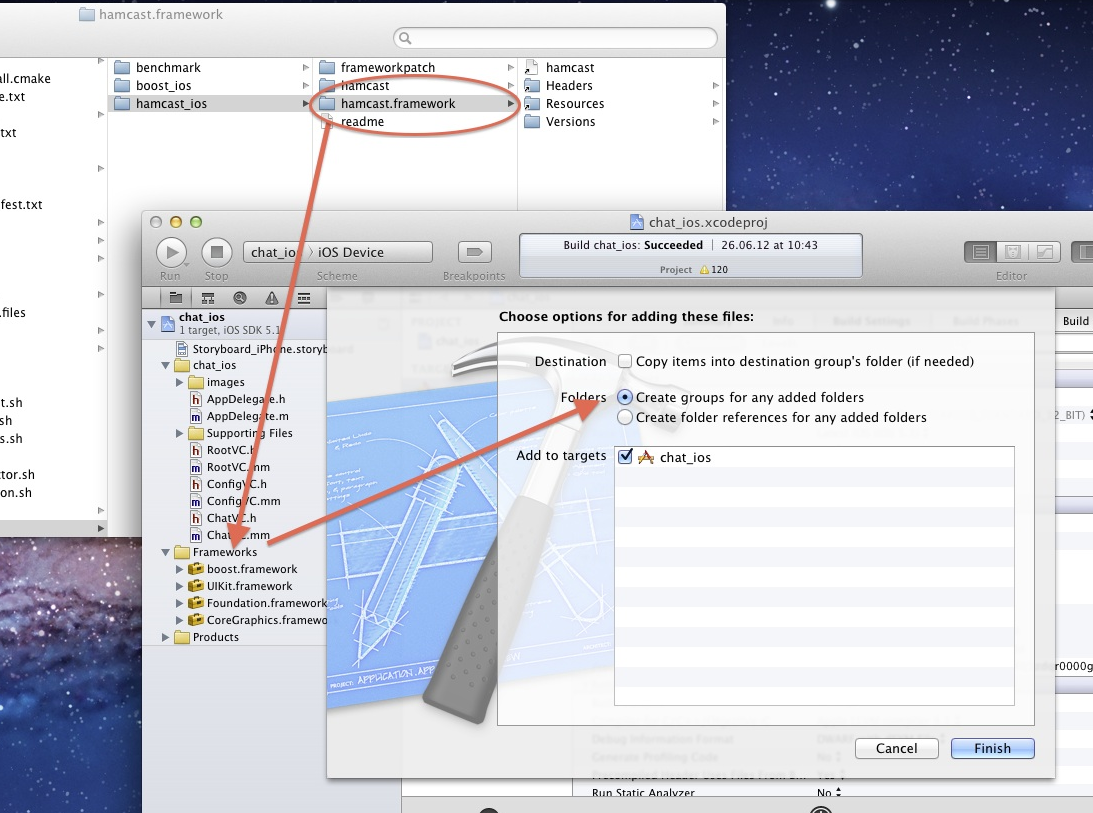
\includegraphics[width=1.0\textwidth]{pictures/import}
%	\caption{Import the the hamcast framework into your project.}
%	\label{fig:import}
%\end{figure}

\section{Use it}
\label{sec:usage}

Hamcast is written in C++. Fortunately you can mix Objective-C, C and C++ in \textit{.mm} files. Rename the ending from \textit{.m} to \textit{.mm} if you want to use hamcast in a class.

The header file for hamcast is named \textit{hamcast.hpp} and should be included as shown below:

\begin{lstlisting}
	#include "hamcast/hamcast.hpp"
\end{lstlisting}

The multicast socket implementation of hamacst is called ``\textit{multicast\_socket}''. As expected the socket provides the functions \lstinline^send^, \lstinline^receive^, \lstinline^join^ and \lstinline^leave^. Hamcast uses ``\textit{URIs}'' as group identifiers, complient with RFC 3986. Both join and leave expect a URI as a parameter. The data you receive with the ``\textit{multicast\_socket}'' is packed in a ``\textit{multicast\_packet}'' and can be obtained via the \lstinline^data()^ and \lstinline^size()^ member functions.

Lets see how this works. The following code is an example function mixing Objective-C and C++. It creates a multicast\_socket, joins a group, interprets received data as strings and prints it on your Xcode console.

\newpage
\begin{lstlisting}
#include "hamcast/hamcast.hpp"
...
	
- (void) receive
{
    hamcast::multicast_socket sck;
	hamcast::multicast_packet message;
    hamcast::uri group("ip://239.255.0.1:30001");
    
    if(group.empty())
    {
        NSLog(@"Not a valid group!");
        return;
    }
    
    sck.join(group);
                       
    while(true)
    {
        message = sck.receive();
        if(message.empty())
        {
            std::cout << "received empty multicast_packet"
            		  << std::endl;
        }
        else
        {
        	std::string output(reinterpret_cast<const char*>
        		(message.data()), message.size());
        	std::cout << "received: " << output << std::endl;
        }
    }
}

...
\end{lstlisting}
\section{Some basics}
\label{sec:tutorial}

\subsection{Heads up}
\label{subsec:headsup}

This is written from our experience, if you are looking for further information the apple developer page~\footnote{https://developer.apple.com/} is quite helpful.

Most Objective-C functions are used diffrently from C and C++ ones. A function call is encapsulated in ``['' and ``]''. In the brackets the object and called function are separated by a blank and arguments are separated from the function via ``:''. Additional arguments have descriptions, which are part of the function name. A function call looks like this:

\begin{lstlisting}
output = [object function:arg1 description:arg2];
\end{lstlisting}

Xcode offers autocompletion for Objective-C functions and thus shows you how to call them correctly.

\subsection{The storyboard}
\label{subsec:storyboard}
In the file tree you should find a ``\textit{.storyboard}'' file. The stroyboard is a way to configure the GUI of your app and specify how your diffrent views are connected. If you click on it, a new view opens in Xcode. At the bottom of the utilies view (the pane on the right side) you can find the object library containing items to use for your app. The default storyboard should contain one view.

\subsubsection{Navigation Controller}
\label{subsubsec:navigationController}
To begin with, use a ``\textit{Navigation Controller}'' to manage your Views. If used, it automatically creates ``\textit{Navigation Bars}'' for your views and buttons to switch back to the previous view. To create it, drag a Navigation Controller from the object library onto the screen. This will create two views, the Navigation Controller on the left and another view. Delete the right one. Your Navigation Controller should be set to be the default View. Select it, head to the ``\textit{attributes inspector}'' tab (found in the utilities pane on the right) and mark the ``\textit{Is initial View Controller}'' option. Since the Navigation Controller does not show up itself, you need to designate a ``\textit{Root View Controller}'' for it. Select the Navigation Controller, right klick it, in the pop-up menu drag the cricle on the right to ``\textit{Relationship - Root View Controller}'' to the target View Controller. See figure~\ref{fig:rootviewcontroller}.

\includeimage{pictures/rootviewcontroller}{Create the Root View Controller Relationship.}{fig:rootviewcontroller}

%\begin{figure}[!h]
%	\centering
%  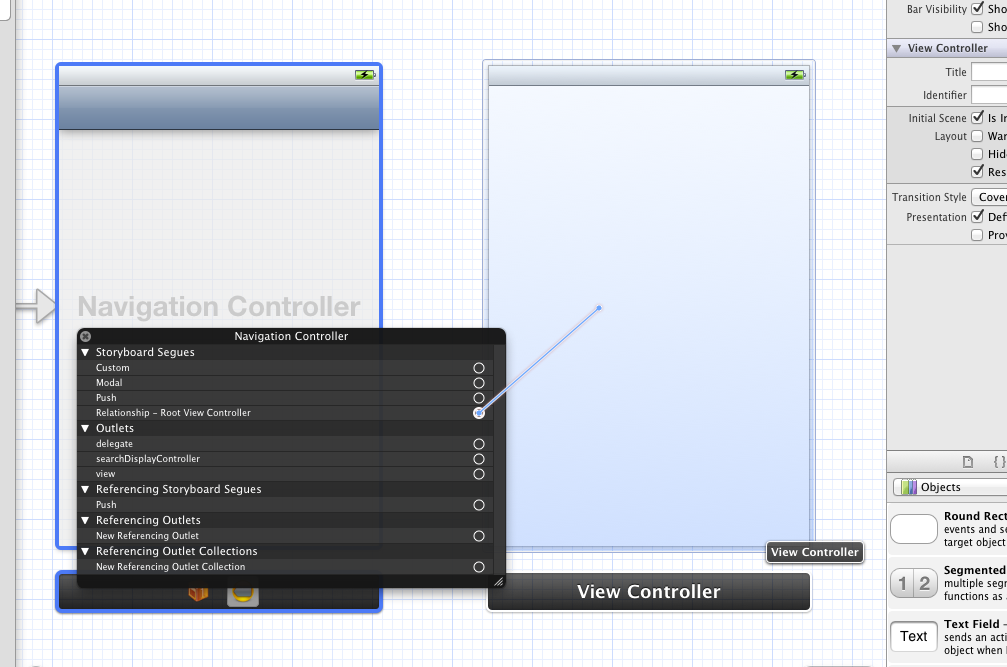
\includegraphics[width=0.9\textwidth]{pictures/rootviewcontroller}
%	\caption{Create the \textit{Root View Controller} Relationship.}
%	\label{fig:rootviewcontroller}
%\end{figure}


\subsubsection{Views}
\label{subsubsec:views}
A view represents a screen with its properties and items. Each view should have its own header and source files (these can be created via \textit{File $\rightarrow$ New $\rightarrow$ File $\rightarrow$ Objective-C class}). You can create a View by dragging a ``\textit{View Controller}'' onto the storyboard screen. Assign a class the view by selecting it and heading to the ``\textit{identity inspector}'' tab. Under ``\textit{Custom Class}'' insert the name of the class.

\subsubsection{Segues}
\label{subsubsec:segues}
If you have multiple views you probably want to switch between those. The storyboard lets you create and name a ``\textit{segue}'' to represent transitions and react to them in your code. If you want to create a segue from A to B, select A and right klick on the top bar of the view. You should see a menu similar to the one from section~\ref{subsubsec:navigationController}. Under Stroyboard Segues drag the circle next to ``\textit{Push}'' onto B. There should now be an arrow between the two views. Click it and name the segue in the ``\textit{attributes identifier}'' tab. See section~\ref{subsubsec:performSegueWithIdentifier} and \ref{subsubsec:prepareForSegue} on how to use a segue in your code.

\subsubsection{Text Fields}
\label{subsubsec:textfields}
To create a text field in your view select the ``\textit{Text Field}'' from the object library and drag it to your view. Go to the header belonging to the view. Open curly brackets after the \lstinline^@interface^ line. Here you can add fields for the class. A text field must have the IBOutlet type, since it is connected  with the interface builder, followed by the type (e.g. \lstinline^UITextField^) and its name. It should now look similar to this:

\begin{lstlisting}
@interface ViewController : UIViewController {
   IBOutlet UITextField *myTF;
}
\end{lstlisting}

To link the text field in your storyboard to the one in your code switch to the storyboard and right klick on the textfield. Drag the ``\textit{delegate}'' circle to the ``\textit{View controller}'' of the assigned class as seen in figure~\ref{fig:textfielddelegate}.
%Do the same for the \textit{New Referencing Outlet} and select the name of your text field (in my case myTF).

Now you can access the text field's text with \lstinline^[myTF text]^. Here is a example how to edit a text field, which is passed as an argument to a function.

\begin{lstlisting}
- (BOOL)textFieldShouldReturn:(UITextField *)textField
{
    if(![@"" isEqualToString:[textField text]])
    {
        NSString *input = [textField text];
        NSLog(@"input:%@", input);
        [textField setText:nil];
    }
    return YES;
}
\end{lstlisting}

This function prints the input to the Xcode console and clears the text field.

\includeimage{pictures/textfielddelegate}{Assign a delegate to a text field.}{fig:textfielddelegate}

%\begin{figure}[!h]
%	\centering
%  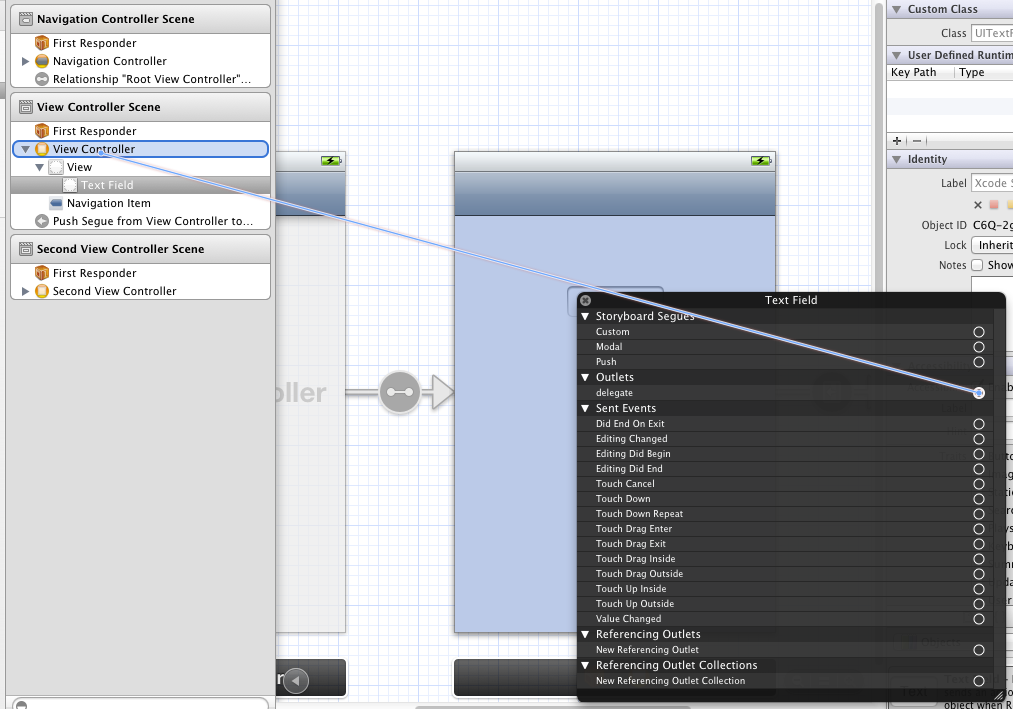
\includegraphics[width=1.0\textwidth]{pictures/textfielddelegate}
%	\caption{Assign a delegate to a text field.}
%	\label{fig:textfielddelegate}
%\end{figure}





\subsection{Useful functions}
\label{subsec:functions}

\subsubsection{\lstinline^- (void) viewDidLoad^}
\label{subsubsec:viewDidLoad}
If you want code to be executed when switched to a view, that code belongs here. It usually already exists and contains the code \lstinline^[super viewDidLoad]^. For example you could start a thread with the \lstinline^receive^ function from section~\ref{sec:usage} here.

\subsubsection{\lstinline^- (BOOL) textFieldShouldReturn:(UITextField *)textField^}
\label{subsubsec:textFieldShouldReturn}
This function is called when return is pressed on the iOS keys. You could hide the keys here with the call \lstinline^[textField resignFirstResponder];^.

\subsubsection{\lstinline^- (void) performSegueWithIdentifier:(NSString *)id sender:(id)sender^}
\label{subsubsec:performSegueWithIdentifier}
Lets you trigger a segue to a diffrent view. The first parameter of this function is the name of the segue you want to trigger. The sender is usually \lstinline^self^;

\subsubsection{\lstinline^- (void) prepareForSegue:(UIStoryboardSegue *)segue sender:(id)sender^}
\label{subsubsec:prepareForSegue}
When a segue is called you can react to the transition in this function. To identify which one is performed use \lstinline^[segue identifier]^. \lstinline{[segue destinationViewController]} gives you  a reference to the next view that can e.g. be used to pass arguments. 

%\subsection{AppDelegate}
%\label{sec:appDelegate}

%\clearpage
%\bibliographystyle{dinat}
%\bibliographystyle{apalike}
%\bibliography{/bib/programming,/bib/rfcs}
%\clearpage
%{\parskip=0mm \listoffigures}
%\clearpage
\end{document}
